\chapter{Simulation}
The activities of the simulation is described in this chapter.
An overview of NS-3 is given, which is then followed by the actions taken, setup
used, assumptions made and overall explanation of the simulation.

\section{NS-3}
A discrete event network simulator, NS-3 is used extensively in network research
and education. The workings and performance of packet data network are modelled
and NS-3 provides a platform for the simulation and experimentation of various
packet-based research. C++ and Python are the predominant language in which NS-3
is written with \textit{waf} as the build system. Design of NS-3 capitalizes on
the object oriented nature of these languages\cite{nsonline}.\\\\
There are various components of packet-based network, fundamentally there are the
endpoint devices, routers,NIC devices ,switches and the medium of exchange.
These components,however in NS-3, are abstracted to reflect what the components
actually do. The endpoint devices are called \textit{Nodes}, exchange medium
- \textit{Channel} and the applications that are generating the packets are 
\textit{Applications} just to name a few. The file/folder structure of a simulation
consist of a model which depicts the fine details of the simulation, a helper that
is supposed to include files containing the installation helper functions, an 
example folder to implement an example of the simulation. There are also doc and 
tests folders and the just as their names suggest they hold documentation and tests
files.\\\\
Installation of the NS-3 is not needed to get a simulation running, as the examples 
or experiments can be run using the binary files gotten from the build process.
It is actually not recommended to do installation of NS-3. Installation in this case
refers to running the command \textbf{\textit{./waf install}}.

\section{Setup}
The simulation was performed on a Gentoo Linux flavor computer with a 64 bit Intel
Eight-Core processor with model name \textit{Intel(R) Core(TM) i7-8565U CPU @
1.80GHz} and RAM of 32GB. Version 3-30 of NS-3 provided the platform on which to
undertake the research. At the time of setting up, this version was the latest most
stable release.\\\\
NS-3 is a voluminous software, the faster processor is needed, as a change to any
file would mean rebuilding the file and its dependencies and those that depend on it.
The version is also critical. Most versions are not backward compartible hence what
works on 3.29 might not work on 3.30 without a little tinkering.\\\\
Gentoo Linux, even though time consuming and quite advance in installation and
setting up, turns to be one of the fastest linux operating systems available. This is
partly due to the fact that source codes are compiled on the host computer with 
specific flags set for optimality.

\section{Components}
For a data packet to move from one endpoint to another, there are components such as,
the packet generating and receiving nodes which will have NIC, the medium(s) through
which the packet traverses also forms a part of the components.\\\\
There are three critical parts, worth mentioning for this simulation; the header which
is attached to the packet, tag-augmented sensor devices and the reader, which, in this
case, is augmented with a server.\\\\
A discussion of the various components follow next.
\subsection{Packet Header}
Various parts of a packet header which is added to a payload enable the packet to get
to its intended destination. A 4-byte(32 bits) header was created, having two fields
of 16 bits each representing the packet type being sent: data packet or broadcast 
and the state of the tag augmented sensor: whether a new data is available for 
transmission or not.\\
\begin{figure}[h!]
\begin{tikzpicture}
    \umlemptyclass[x=0,y=0]{Header}{
}{}
\umlclass[x=5.5,y=-2]{AptMacHeader}{
  -m\_id : uint16\_t \\ -m\_type : uint16\_t \\ -m\_stateChange : uint16\_t
}{
  +AptMacHeader() \\ +SetId(id : uint16\_t) : void \\ +GetId (void) : const
  uint16\_t\\ +SetPacketType(ptype : uint16\_t) : void \\ +GetPacketType(void) :
  const uint16\_t \\ +SetStateChange(stateChange : uint16\_t) : void \\ 
  +GetStateChange(void) : const uint16\_t \\ \umlstatic{+GetTypeId(void) : TypeId}\\
  \umlvirt{+Serialize(start : Buffer::Iterator) : const void} \\
  \umlvirt{+Deserialize(start : Buffer::Iterator) : uint32\_t} \\
  \umlvirt{+GetSerializedSize(void) : const uint32\_t} \\
  \umlvirt{+GetInstanceTypeId (void) : const TypeId} \\
  \umlvirt{+Print(\&os : std::ostream) : const void}\\
}
\umlenum[x=12.5,y=-4]{HeaderContents}{
    BROADCAST : uint16\_t \\ DATA : uint16\_t \\ STATECHANGE : uint16\_t
}

%\umlassoc[geometry=-|-, arg1=tata, mult1=*, pos1=0.3, arg2=toto, mult2=1, pos2=2.9, align2=left]{C}{Header}
%\umlunicompo[geometry=-|, arg=titi, mult=*, pos=1.7, stereo=vector]{D}{C}
%\umlimport[geometry=|-, anchors=90 and 50, name=import]{sp2}{sp1}
\umlaggreg[geometry=-|]{AptMacHeader}{HeaderContents}
\umlinherit[geometry=-|]{AptMacHeader}{Header}
%\umlnote[x=2.5,y=-6, width=3cm]{B}{Je suis une note qui concerne la classe B}
%\umlnote[x=7.5,y=-2]{import-2}{Je suis une note qui concerne la relation d'import}
\end{tikzpicture}
\caption{APT-MAC Header UML}
\label{fig:headerUML}
\end{figure}\\
The UML class diagram is illustrated in Figure \ref{fig:headerUML}. The \emph{
constructor, getter and setter} functions are for their usual purposes. \emph{
Serialize} function puts the various fields of the header in series by writing them
from host-order to network-order and the \emph{Deserialize} reads from network-order
to host-order. \emph{Enum HeaderContents} holds the value of the various fields of
the header.


\subsection{Tag Augmented Sensor Devices}
Devices in a smart home are broadly classified under three categories: periodic
(e.g., temperature sensors), real-time (e.g., joystick, cameras) and event based 
(e.g., presence detector, remote of appliances)\cite{Maselli}. The state changes
of the various devices were modelled according to Markov Chains\cite{Tolver}.
\begin{figure}[h]
    \begin{subfigure}[b]{.5\textwidth}
        \centering
        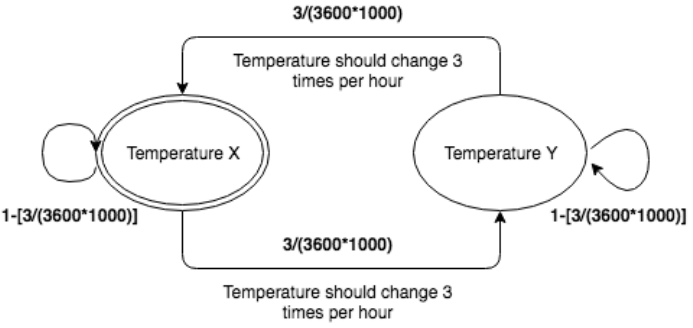
\includegraphics[width=1\linewidth]{temperature-sensor}
        \caption{Temperature Sensor model}
        \label{fig:temperature-sensor}
    \end{subfigure}
    \begin{subfigure}[b]{.5\textwidth}
        \centering
        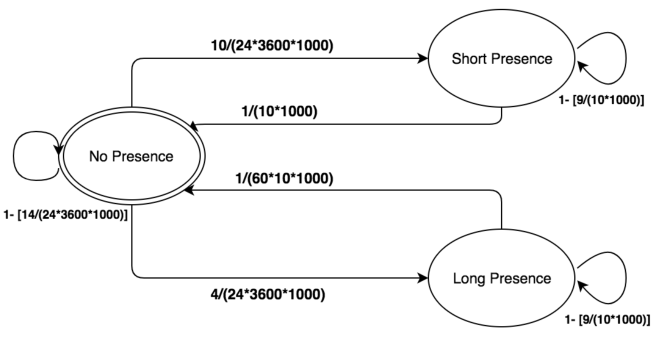
\includegraphics[width=1\linewidth]{presence-sensor}
        \caption{Presence Sensor model}
        \label{fig:presence-sensor}
    \end{subfigure}
    \begin{subfigure}[b]{.5\textwidth}
        \centering
        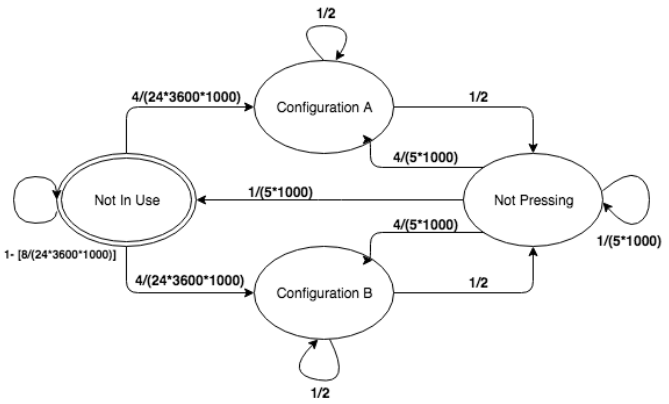
\includegraphics[width=1\linewidth]{tv-remote}
        \caption{TV Remote model}
        \label{fig:tv-remote}
    \end{subfigure}
    \begin{subfigure}[b]{.5\textwidth}
        \centering
        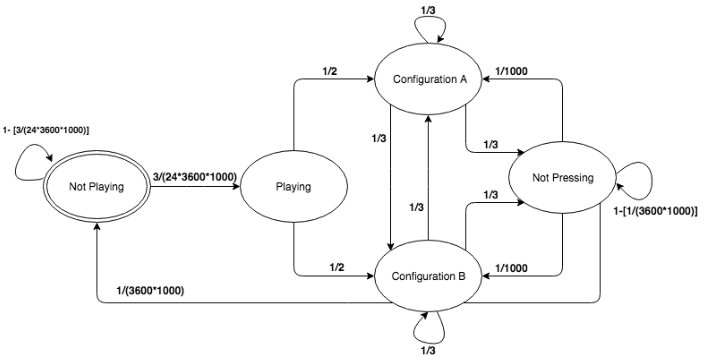
\includegraphics[width=1\linewidth]{joysick-sensor}
        \caption{Joystick model}
        \label{fig:joysick-sensor}
    \end{subfigure}
\end{figure}
Figures \ref{fig:temperature-sensor} to \ref{fig:joysick-sensor}, taken from
\cite{Maselli}, depicts the transition probabilities of the various states a device
could be in. The state change is based on time. Taking fig \ref{fig:temperature-sensor}
for instance, it was found that a temperature sensor produces new data three times in
an hour hence the various probabilities with respect to time in milliseconds.\\\\
